\documentclass[11pt]{article}
\usepackage{graphicx}
\usepackage{amsmath}
\usepackage{siunitx}
\usepackage[super]{nth}
\usepackage{caption}
\usepackage{parskip}
\usepackage{placeins}
\usepackage[hidelinks]{hyperref}
%\usepackage[nottoc,numbib]{tocbibind}

%\usepackage{hyperref}

\title{Investigation on Relationship Between Location of Fretted Note on Guitar Neck and Note Intonation Error.}
\author{IB Physics Extended Essay}
\date{March 12, 2023 \\~\\\tiny Word Count: 3997}

\begin{document}
    \maketitle
    \newpage
    \tableofcontents
    \newpage
    \begin{flushleft}
    \section{Introduction}
        \subsection{Personal observation}
            Music and sound have always held a special place in my heart, not only as a form of entertainment but also as a means of self-expression and creativity. Since a very young age, I have been fascinated with and have pursued stringed instruments like basses and guitars. Through playing these instruments, I have been able to explore the different components of music and sound, and have developed a keen ear for tone and texture. However, recently I have become increasingly aware of the importance of intonation, which refers to the accuracy of the instrument's pitch across all frets. While playing the guitar, I have noticed that even slight deviations in intonation can have a significant impact on the overall sound quality. This change in intonation often starts around fret 7-8 and above, and most noticeable especially when I play chords high up the neck with a distortion pedal. This is because the higher harmonic frequencies from the distortion will clash with the other notes in the chord when the intonation is not perfect. This will result in a very muffled, discordant sounding chord. This intonation problem has been a topic of debate in many guitar forums online, with a lot of hypotheses on why it happens and discussions on how to set a perfect intonation. Therefore this motivated me to combine it with my love of physics and investigate the principles behind this problem. I want to explore how intonation works, why the note intonation is “off” when you fret a string on high frets, and from there propose solutions to achieve perfect intonation. This investigation is not only significant for my hobby of playing the guitar, but it is also a topic of interest for many musicians and music lovers worldwide. By delving deeper into the science behind the intonation, I hope to not only improve my skills as a guitarist but also contribute to the broader community of music enthusiasts.
        \subsection{Background information \& Theory}
            \subsubsection*{Basic model of guitar strings and frets}
                The most simple model of an electric guitar basically consists of a piece of steel string anchored at two ends by the bridge saddle and the nut. One end is usually wrapped around a tuning peg to make the string tension adjustable to tune the string to a certain frequency. This is stretched over a pickup to capture the string vibrations and turn it into electrical signals, and a fretboard with raised metal frets. The fret distances are carefully calculated and accurately placed along the length of the string, so that when the string is pressed down on a fret, the fret itself will act as a stopper and change the length of the vibrating string, thereby changing the vibrating frequency to make other notes in a scale. 
                \begin{figure}[h]
                    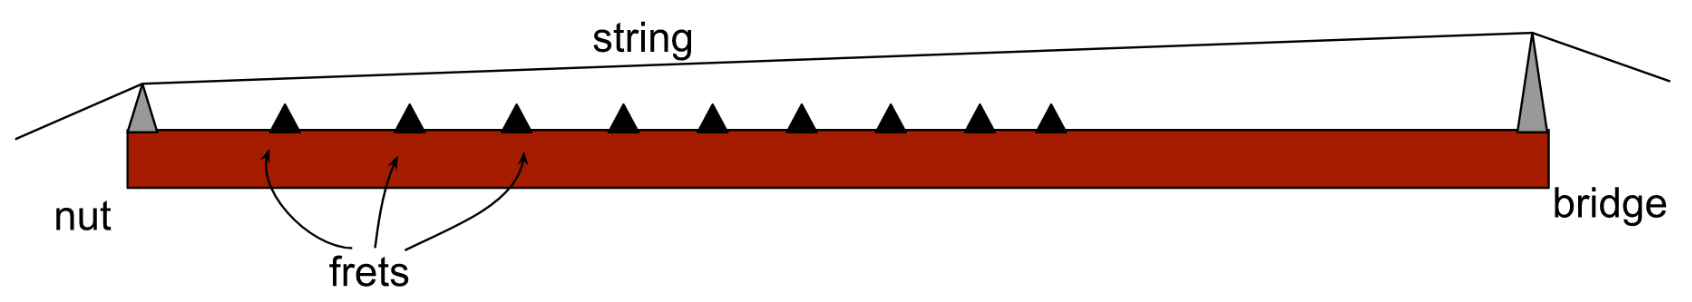
\includegraphics[width=\textwidth]{fig1.png}
                    \caption{A simplified model of the electric guitar I will use. The pickup has been removed.}\label{fig1}
                \end{figure} 
                \FloatBarrier
            \subsubsection*{How the guitar string produces sound}
                When the string is plucked, it will create travelling waves on the string that reflect at both ends, creating standing waves. The frequency of the standing waves with the longest wavelength is the fundamental frequency, also called the first harmonic. This is the lowest frequency, and there will usually be other higher harmonics that when combined together create the characteristic timbre of the electric guitar. 
                \begin{figure}[h]
                    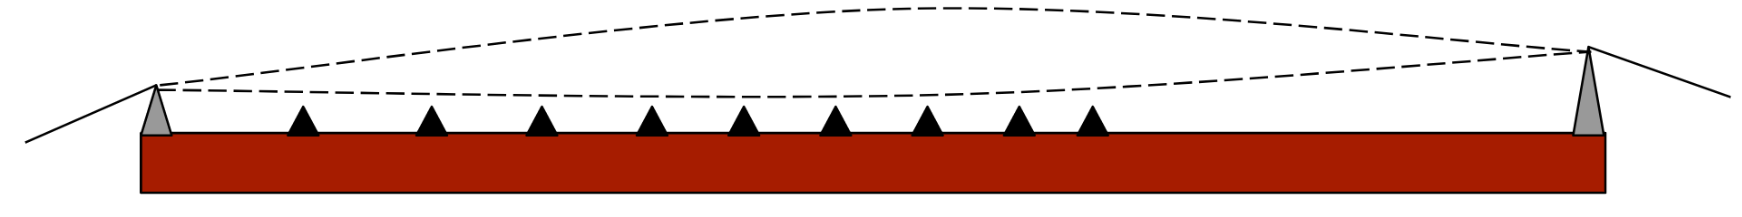
\includegraphics[width=\textwidth]{fig2.png}
                    \caption{The “open” string (not fretted) is plucked and vibrating at its fundamental frequency.}\label{fig2}
                \end{figure} 
            
                The fundamental frequency $f_0$ of a string is determined by this formula
                \begin{equation}\label{eqn1}
                    f_0 = \frac{v}{\lambda}
                \end{equation}
                where $v$ is the speed of the wave on the string and $\lambda$ is the wavelength. \cite{eqn1} \par 
                From Figure \ref{fig2} we see the wavelength is double the length of the guitar - the “scale length” $l$ . Therefore \begin{equation}\label{eqn2}
                    \lambda = 2l
                \end{equation}
                The speed of the wave $v$ on a stretched string with tension $T$ can be determined by the equation:
                \begin{equation}\label{eqn3}
                    v = \sqrt{\frac{T}{\mu}} 
                \end{equation}
                Where $\mu$ is the linear density of the string (mass of string per unit length) \cite{eqn3}\par
                Substitute (\ref{eqn2}) and (\ref{eqn3}) into (\ref{eqn1}) we get the expression for the frequency of an open string
                \begin{equation}\label{eqn4}
                    f_0 = \frac{1}{2l}\sqrt{\frac{T}{\mu}}
                \end{equation}

            \subsubsection*{How frets work}
                When the string is pressed down on a fret and plucked, its vibrating length changes which  changes the frequency as well.\par
                Let's say we press down on fret $n$. The distance from the saddle to the fret then is $l_n$
                
                \begin{figure}[!ht]
                    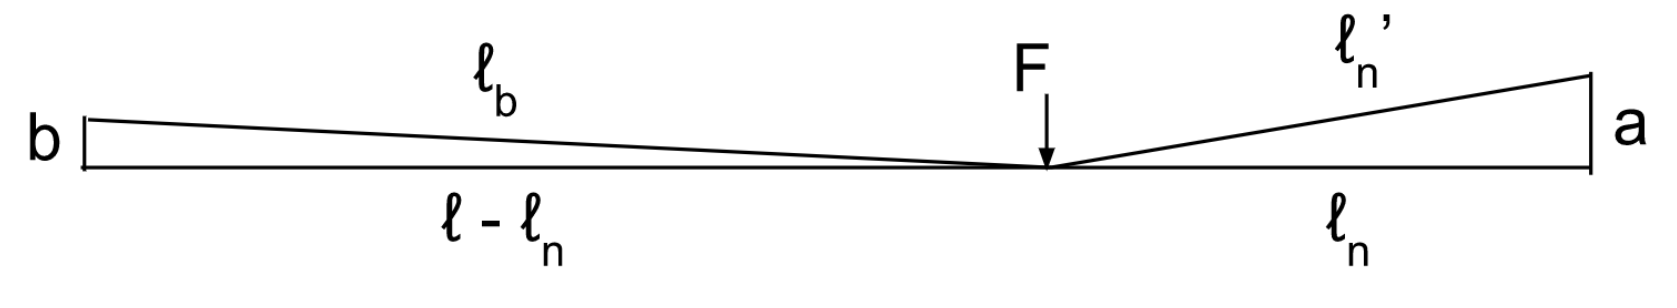
\includegraphics[width=\textwidth]{fig3.png}
                    \caption{A simplified model of the fretted string}\label{fig3}
                \end{figure} 

                Theoretically, the frequency of this note is 
                \begin{equation}\label{eqn5}
                    f_n = \frac{1}{2l_n}\sqrt{\frac{T}{\mu}}
                \end{equation}

                In order to make the frequency match with a specific note in the Western twelve-tone equal temperament (12-TET) system, the scale length needs to be divided into powers of $\sqrt[12]{2}$. To do this luthiers traditionally use a formula to calculate the position of each fret. \cite{eqn6}

                \begin{equation}\label{eqn6}
                    l_n=\frac{l}{2^\frac{n}{12}}
                \end{equation}
            
            \subsubsection*{Cause of intonation issues}
                When pressed down, due to the distance between the nut and the saddle to top of the frets ($b$ and $a$ respectively in Figure \ref{fig3}), the vibrating string length also stretches. The effective vibrating length is now $l_n'$. The fretting force $F$ also causes an increase in tension of the whole string, so the tension now is $T+ \Delta T$. \par
                Therefore, taking into account the fretting action, the frequency now will no longer be the same as the intended frequency $f_n$. This explains why we observe the intonation problem when fretting down on the string. We will call this new frequency $f_n'$
                \begin{equation}\label{eqn7}
                    f'_n= \frac{1}{2l_n'}\sqrt{\frac{T+\Delta T}{\mu}}
                \end{equation}
                
                The intonation deviation is then simply
                \begin{align}
                    \Delta f &= f_n'-f_n \\
                    &= \frac{1}{2\sqrt{\mu}} \left( \frac{\sqrt{T+\Delta T}}{l_n'} - \frac{\sqrt{T}}{l_n} \right)\label{eqn9}
                \end{align}
                
                From Figure \ref{fig3}, using Pythagoras' Theorem for $l_n'$ we get
                \begin{align}
                    l_n' &= \sqrt{l_n^2+a^2} \\
                    &= \sqrt{l_n^2\left(1+\left(\frac{a}{l_n}\right) ^2\right)} \\
                    &= l_n \sqrt{1+\left(\frac{a}{l_n}\right) ^2} \\
                    &= l_n \left(1+\left(\frac{a}{l_n}\right) ^2\right)^{\frac{1}{2}} 
                \end{align}
                Subbing this into (\ref{eqn9}):
                \begin{align}
                    \Delta f &= \frac{1}{2\sqrt{\mu}} \left( \frac{\sqrt{T+\Delta T}}{l_n\sqrt{1+\left(\frac{a}{l_n}\right) ^2}} - \frac{\sqrt{T}}{l_n} \right) \\
                    &= \frac{1}{2l_n\sqrt{\mu}} \left( (T+\Delta T)^{\frac{1}{2}} \left( 1+\left(\frac{a}{l_n}\right) ^2\right)^{-\frac{1}{2}} - \sqrt{T} \right) \\
                    &= \frac{1}{2l_n\sqrt{\mu}} \left( T^{\frac{1}{2}}\left(1+\frac{\Delta T}{T}\right)^{\frac{1}{2}} \left( 1+\left(\frac{a}{l_n}\right) ^2\right)^{-\frac{1}{2}} - \sqrt{T} \right) \\
                    &= \frac{1}{2l_n} \sqrt{\frac{T}{\mu}}\left(\left(1+\frac{\Delta T}{T}\right)^{\frac{1}{2}} \left( 1+\left(\frac{a}{l_n}\right) ^2\right)^{-\frac{1}{2}} - 1 \right)
                \end{align}

                Since $\Delta T$ is much smaller than T, and similarly $a$ is much smaller than $l_n$, we can approximate this to the first order
                \begin{align}
                    \Delta f &\approx \frac{1}{2l_n} \sqrt{\frac{T}{\mu}} \left( \left(1+\frac{\Delta T}{2T}\right) \left( 1- \frac{a^2}{2{l_n}^2} \right) - 1\right)\label{eqn18} \\ 
                    &= \frac{1}{2l_n} \sqrt{\frac{T}{\mu}} \left( -\frac{a^2}{2{l_n}^2} + \frac{\Delta T}{2T} - \frac{a^2\Delta T}{4T{l_n}^2}\right) \\
                    &\approx \frac{1}{4l_n} \sqrt{\frac{T}{\mu}} \left( \frac{\Delta T}{T} - \frac{a^2}{{l_n}^2} \right) \label{eqn20}
                \end{align}

            \subsubsection*{Tension of the guitar string}
                A stretched guitar string is under tension $T$. When we press down on it, the whole string stretches accordingly by a small amount $\Delta l$. Assuming there is no friction on the point of contact, the tension in the whole string increases by an amount $\Delta T$, determined by:
                \begin{equation}
                    \Delta T = \frac{AY\Delta l}{l}\label{eqn21}
                \end{equation} 
                Where $A$ is the cross sectional area of the string, and $Y$ is the Young's modulus of the material. \cite{polak} \par
                The total amount of stretch of the string $\Delta l$ can be calculated from Figure \ref{fig3}. 
                \begin{align}
                    \Delta l &= (l_b + l_n') - l \\
                    &= \sqrt{(l-l_n)^2+b^2} + \sqrt{l_n^2+a^2} - l \\
                    &= (l-l_n)\sqrt{1+\left(\frac{b}{l-l_n}\right)^2} + l_n\sqrt{1+\left(\frac{a}{l_n}\right)^2} - l\\
                    &= (l-l_n)\left(1+\left(\frac{b}{l-l_n}\right)^2\right)^{\frac{1}{2}} + l_n\left(1+\left(\frac{a}{l_n}\right)^2\right)^{\frac{1}{2}} - l
                \end{align}
                Once again, we can approximate this to the first order since both $a$ and $b$ are much smaller than $l_n$ and $l-l_n$. Therefore,
                \begin{align}
                    \Delta l &\approx (l-l_n)\left(1+\frac{b^2}{2(l-l_n)^2}\right)+ l_n\left(1+\frac{a^2}{2l_n^2}\right) - l \label{eqn26} \\
                    &= (l - l_n) + \frac{b^2}{2(l-l_n)} + l_n + \frac{a^2}{2l_n} - l \\
                    &= \frac{b^2}{2(l-l_n)} + \frac{a^2}{2l_n}
                \end{align}
                Substituting this into (\ref{eqn21}) we get
                \begin{equation}
                    \Delta T = \frac{AY}{2l} \left( \frac{b^2}{l-l_n} + \frac{a^2}{l_n} \right) \label{eqn29}
                \end{equation}

            \subsubsection*{Final expression relating frequency change and position of fret}
                Finally, we can substitute (\ref{eqn29}) into (\ref{eqn20}) to get the expression between the intonation shift $\Delta f$ and the fret position $l_n$
                \begin{align}
                    \Delta f &= \frac{1}{4l_n} \sqrt{\frac{T}{\mu}} \left( \frac{AY}{2Tl} \left( \frac{b^2}{l-l_n} + \frac{a^2}{l_n} \right) - \frac{a^2}{{l_n}^2} \right) \label{eqn30}
                \end{align}
                From (\ref{eqn4}) we get
                \begin{equation*}
                    \sqrt{\frac{T}{\mu}} = 2lf_0
                \end{equation*}
                and 
                \begin{equation*}
                    T = 4\mu l^2{f_0}^2    
                \end{equation*}
                Subbing into (\ref{eqn30})
                \begin{equation}
                    \Delta f = \frac{l f_0}{2l_n} \left( \frac{AY}{8\mu l^3 {f_0}^2} \left( \frac{b^2}{l-l_n} + \frac{a^2}{l_n} \right) - \frac{a^2}{{l_n}^2} \right) \label{eqn31}
                \end{equation}
                $\mu$, the linear density of the string, is simply the mass per unit length of the string:
                \begin{equation*}
                    \mu = \frac{m}{l} = \frac{\rho V}{l} = \frac{\rho l A}{l} = \rho A
                \end{equation*}
                where $m$ is the mass of the vibrating string section, $V$ is its volume, and $\rho$ is the volumetric density of the material. Subbing this into (\ref{eqn31}):
                \begin{align}
                    \Delta f &= \frac{l f_0}{2l_n} \left( \frac{AY}{8\rho A l^3 {f_0}^2} \left( \frac{b^2}{l-l_n} + \frac{a^2}{l_n} \right) - \frac{a^2}{{l_n}^2} \right) \label{eqn32} \\
                    &= \frac{l f_0}{2l_n} \left( \frac{Y}{8\rho l^3 {f_0}^2} \left( \frac{b^2}{l-l_n} + \frac{a^2}{l_n} \right) - \frac{a^2}{{l_n}^2} \right) \label{eqn33}
                \end{align}

    \section{Experiment}
        From the final expression relating $\Delta f$ and $l_n$, knowing all other constants I can plot the graph for this. $\Delta f$ is the dependent variable, and $l_n$ is the independent variable. I expect the intonation difference $\Delta f$ to be higher when the fretting distance is closer to the bridge ($l_n$ closer to 0), and lower closer to the nut, in the first few frets (larger values of $l_n$). The general shape of the graph can be compared with my expectation as a sanity check. It is impossible to linearize the equation, therefore I will have to resort to collecting the data, plotting the graph, then confirming the relationship using a regression method to see how well the data fits the model. \par
        The choice of guitar I will use for this experiment is a Fender Stratocaster. This is arguably the most iconic and popular guitar in history, known for its versatility and playability. Therefore I pick this guitar because there is a wealth of information available on it, to make it easier to find data to support my research or to compare my results to other studies. Also this will make it easier to control variables in my experiment and ensure consistent results. Another benefit is to ensure ease of replicability of the experiment. \par
        The choice of string I will use is a G string from D'Addario's set of Nickel Wound Regular Light Gauge - EXL110-10P that I have at home. I choose the G string because it is the thickest string in the set that is a plain unwound string. This is because from my experience the thicker strings will make the effects of the intonation shift more noticeable. %cite this
        \subsection{Determining the constants}
            From the equation (\ref{eqn33}), the constants I need to determine are $f_0$, $\rho$, $Y$, $a$, $b$ and $l$. 
            \begin{itemize}
                \item $l$ is the scale length of the guitar. For a Fender Stratocaster, it is 25.5 inches (64.77cm). \cite{scale} I round this up to 64.8cm (3s.f). From this information, I can adjust the bridge saddle position so that the scale length matches 64.8cm (0.648 m)
                \item Initial frequency $f_0$ can be measured directly in the experiment. The frequency we aim for is the frequency of G string on the guitar for a standard A440 tuning system, $G_3$ at 196 Hz \cite{freq_chart}
                \item Young's modulus $Y$ is dependent on the specifications of the string material. Nearly all electric guitar strings follow the ASTM-A228 manufacturing standards for steel music wire, and the value of $Y$ is \SI{210}{\giga\pascal} (\SI{2.10e11}{\pascal}). \cite{astm} 
                \item $\rho$, the density of the string material, is determined according to the ASTM-A228 standards. $\rho = \SI{7.80e3}{\kg.m^{-3}}$. \cite{astm}
                \item $a$ and $b$: it is very hard to measure these directly, as they are distance from the nut and saddle to the top of the fret, not the height itself. Therefore I can only set up the guitar indirectly according to recommended values and calculate them afterwards. There are a lot of resources online on how to set up the guitar. I choose to follow the instructions by Stewmac \cite{stewmac}, a reputable online guitar retailer, and take the average value of the action (distance between string and top of fret) for the \nth{1} fret to be 0.016" (0.406mm) and \nth{12} fret to be 0.070" (1.78mm). I change the adjustable saddle height and file down/shim up the nut height to match these values. From there I can calculate the values of $a$ and $b$ as illustrated by Figure \ref{fig4}: \par
                \begin{figure}[ht]
                    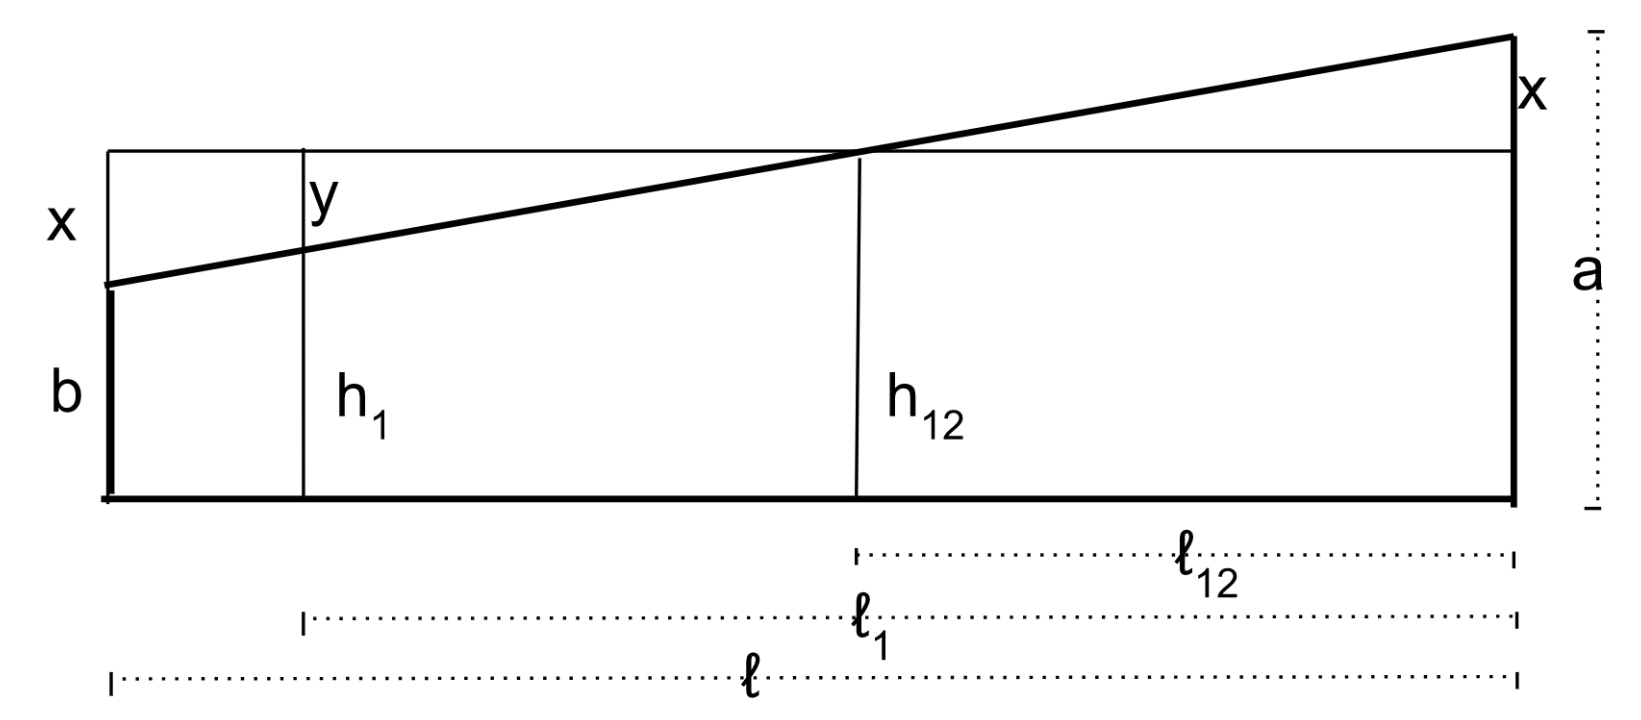
\includegraphics[width = \textwidth]{fig4.png}
                    \caption{Diagram to calculate values of $a$ and $b$ (Exaggerated)} \label{fig4}
                \end{figure}
                \FloatBarrier
                Since fret \nth{12} is exactly in the middle of l ($l_{12} = \frac{l}{2} = \frac{.648}{2} = .324$ m) we get a pair of congruent triangles as highlighted. Therefore:
                \begin{align*}
                    a &= h_{12} + x \\
                    b &= h_{12} - x
                \end{align*}
                From the luthier formula (\ref{eqn6}) we get
                \begin{align*}
                    l_1 &= \frac{l}{2^{\frac{1}{12}}} \\
                        &= \frac{.648}{2^{\frac{1}{12}}} \\
                        &= \SI{.612}{\meter}
                \end{align*}
                and we also get the ratio in Figure \ref{fig4}
                \begin{align*}
                    \frac{x}{y} &= \frac{l-l_{12}}{l_1-l_{12}} \\
                    x &= y\frac{l-l_{12}}{l_1-l_{12}} \\
                    &= (h_{12}-h_1)\frac{l-l_{12}}{l_1-l_{12}} \\
                    &= (1.78-.406) \cdot 10^{-3} \cdot \frac{.648-.324}{.612-.324} \\
                    &= \SI{1.55e-3}{\meter}
                \end{align*}
                Therefore
                \begin{align*}
                    a &= 1.78 + 1.55 = \SI{3.33e-3}{\meter} \\
                    b &= 1.78 - 1.55 = \SI{1.30e-4}{\meter}
                \end{align*}    
            \end{itemize}

        \subsection{Apparatus}
            \begin{itemize}
                \item 1 Fender Stratocaster style guitar
                \item 1 17-gauge plain unwound steel G string
                \item 1 guitar capo 
                \item 1 guitar pick
            \end{itemize}
        \subsection{Process}
            \begin{enumerate}
                \item Setting up the guitar. I used the instructions by Stewmac \cite{stewmac}
                \item Connect the guitar to frequency measuring software. I used my audio interface to connect the guitar to my laptop, and the software I used is Visual Analyzer 2020 \cite{va20}. I choose this because it supports Fast Fourier Transform in real-time to convert guitar signals into frequency spectrum, and can be configured to provide results with high accuracy. 
                \item Measure $f_0$ by plucking the string with no capo on.
                \item Pluck it 5 times with the pick, changing the plucking position each time (above the neck pickup, between neck and middle, above middle, between middle and bridge, and above bridge pickup). Record the peak frequency (highest dB) for each pick. \label{enum4}
                \item Put capo on \nth{7} fret and repeat step \ref{enum4}. Ensure that the edge of the capo must be right on top of the fret and the capo is pushing the string straight downwards, not sideways. (Figure \ref{fig6})\label{enum5}
                \item Repeat step \ref{enum5} from fret 8 up to fret 16. I cannot go higher than this because this is where the neck meets the body, it is impossible to put the capo.
            \end{enumerate}
            \newpage
            \subsubsection*{Photos of experimental set up}
                \FloatBarrier
                \begin{figure}[!htb]
                    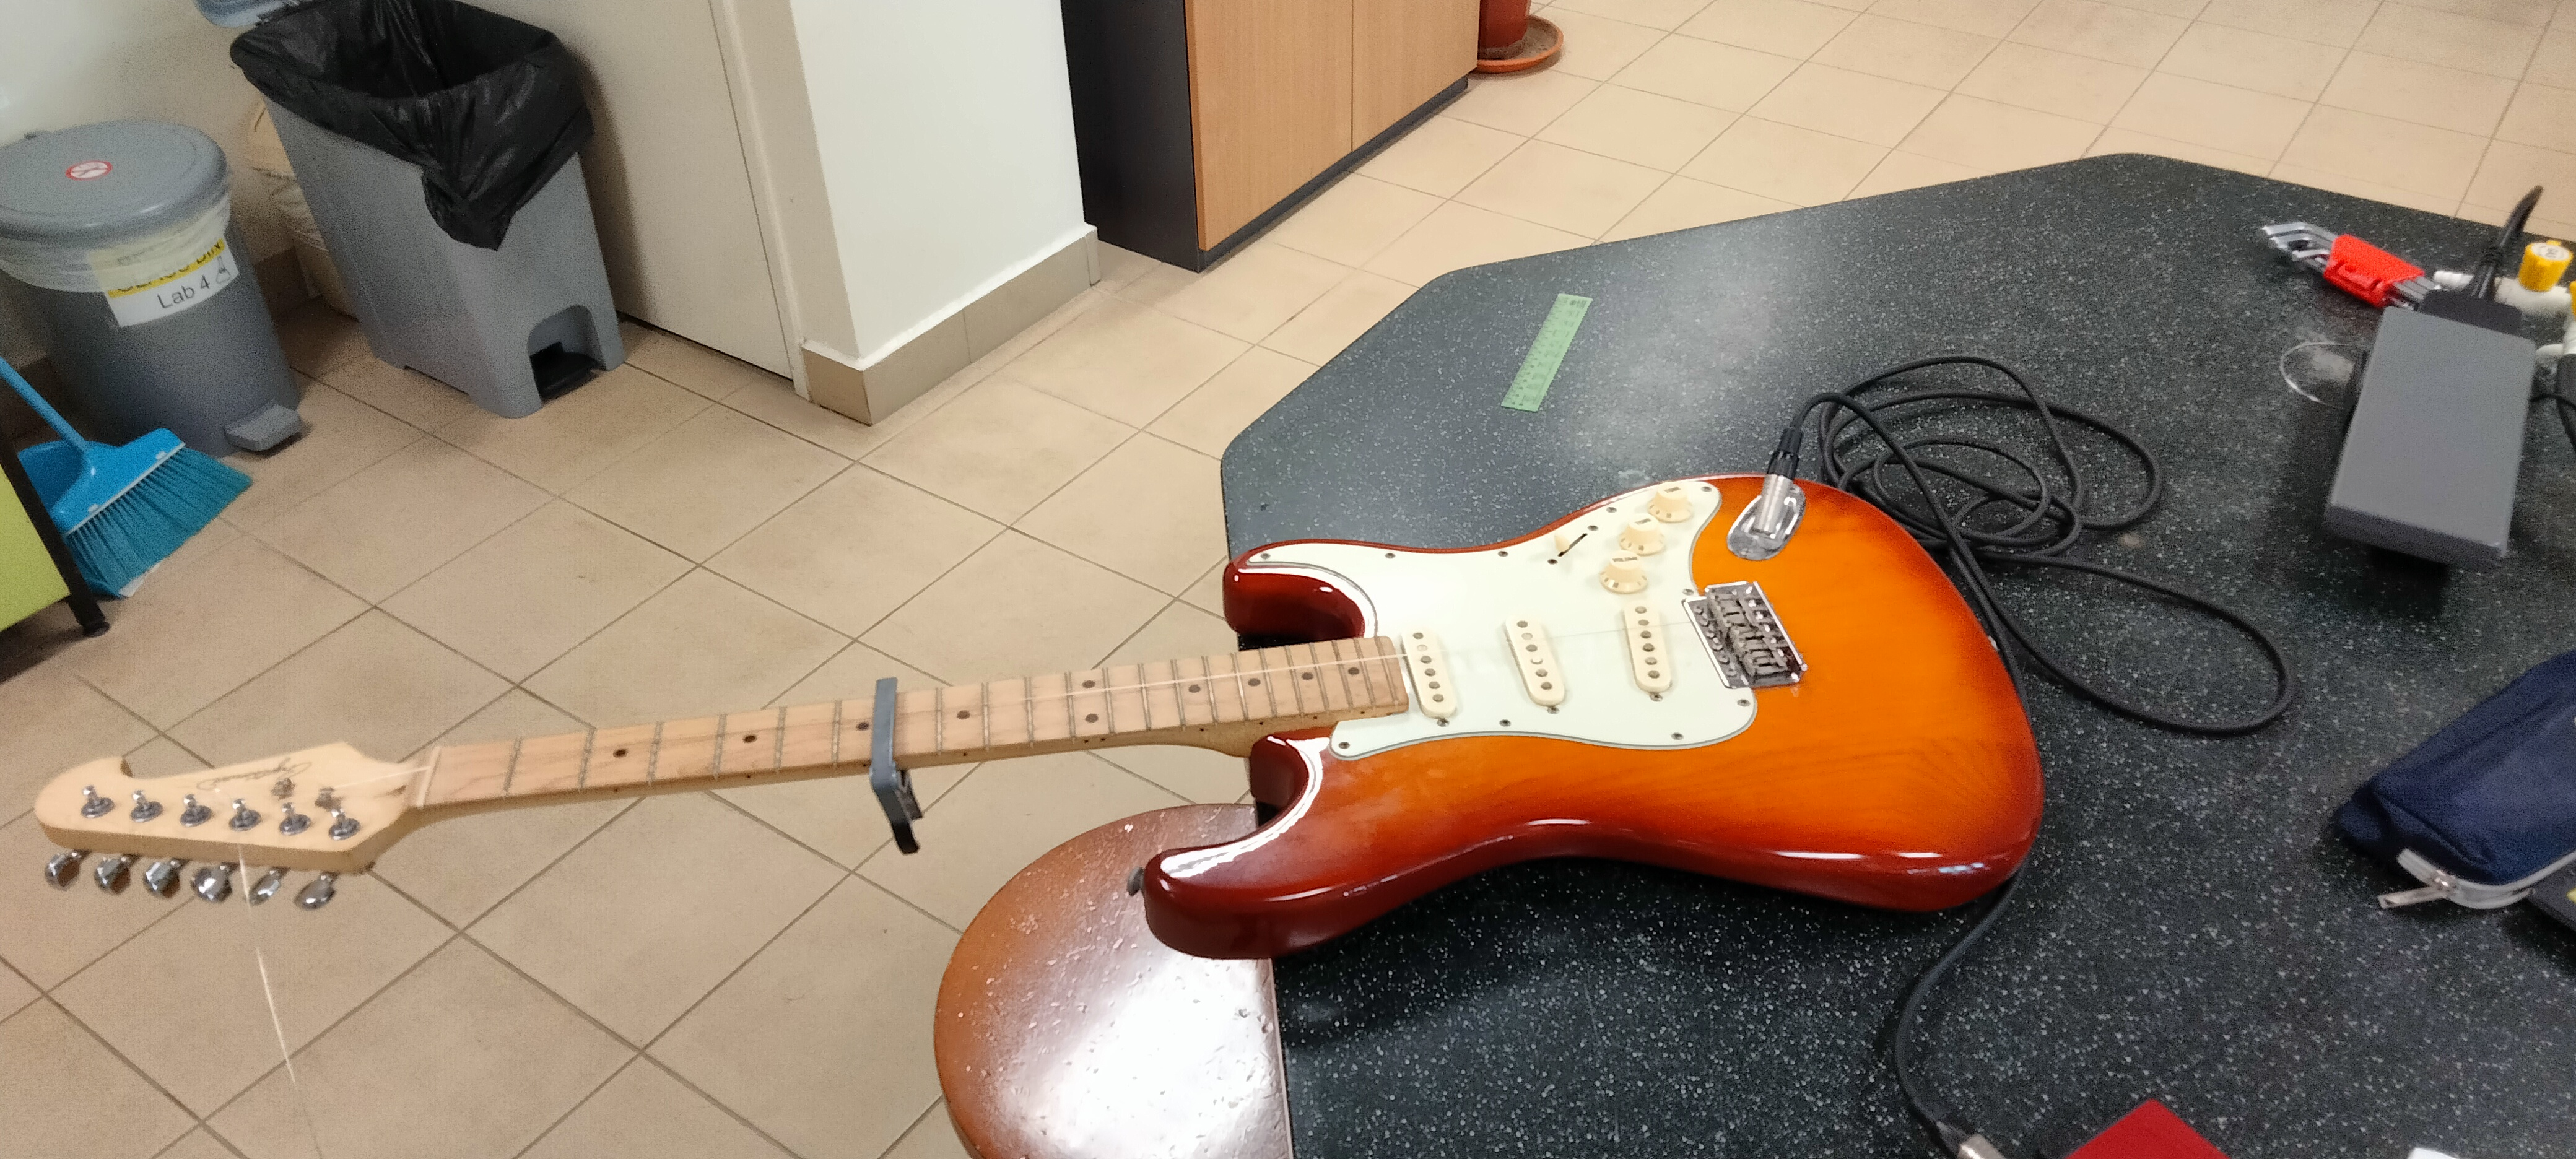
\includegraphics[width = \textwidth]{ee/experiment_setup.jpg}
                    \caption{My experimental setup. I position the guitar neck outside the table for ease of access to the capo} \label{fig5}
                \end{figure}
                \begin{figure}[!htb]
                    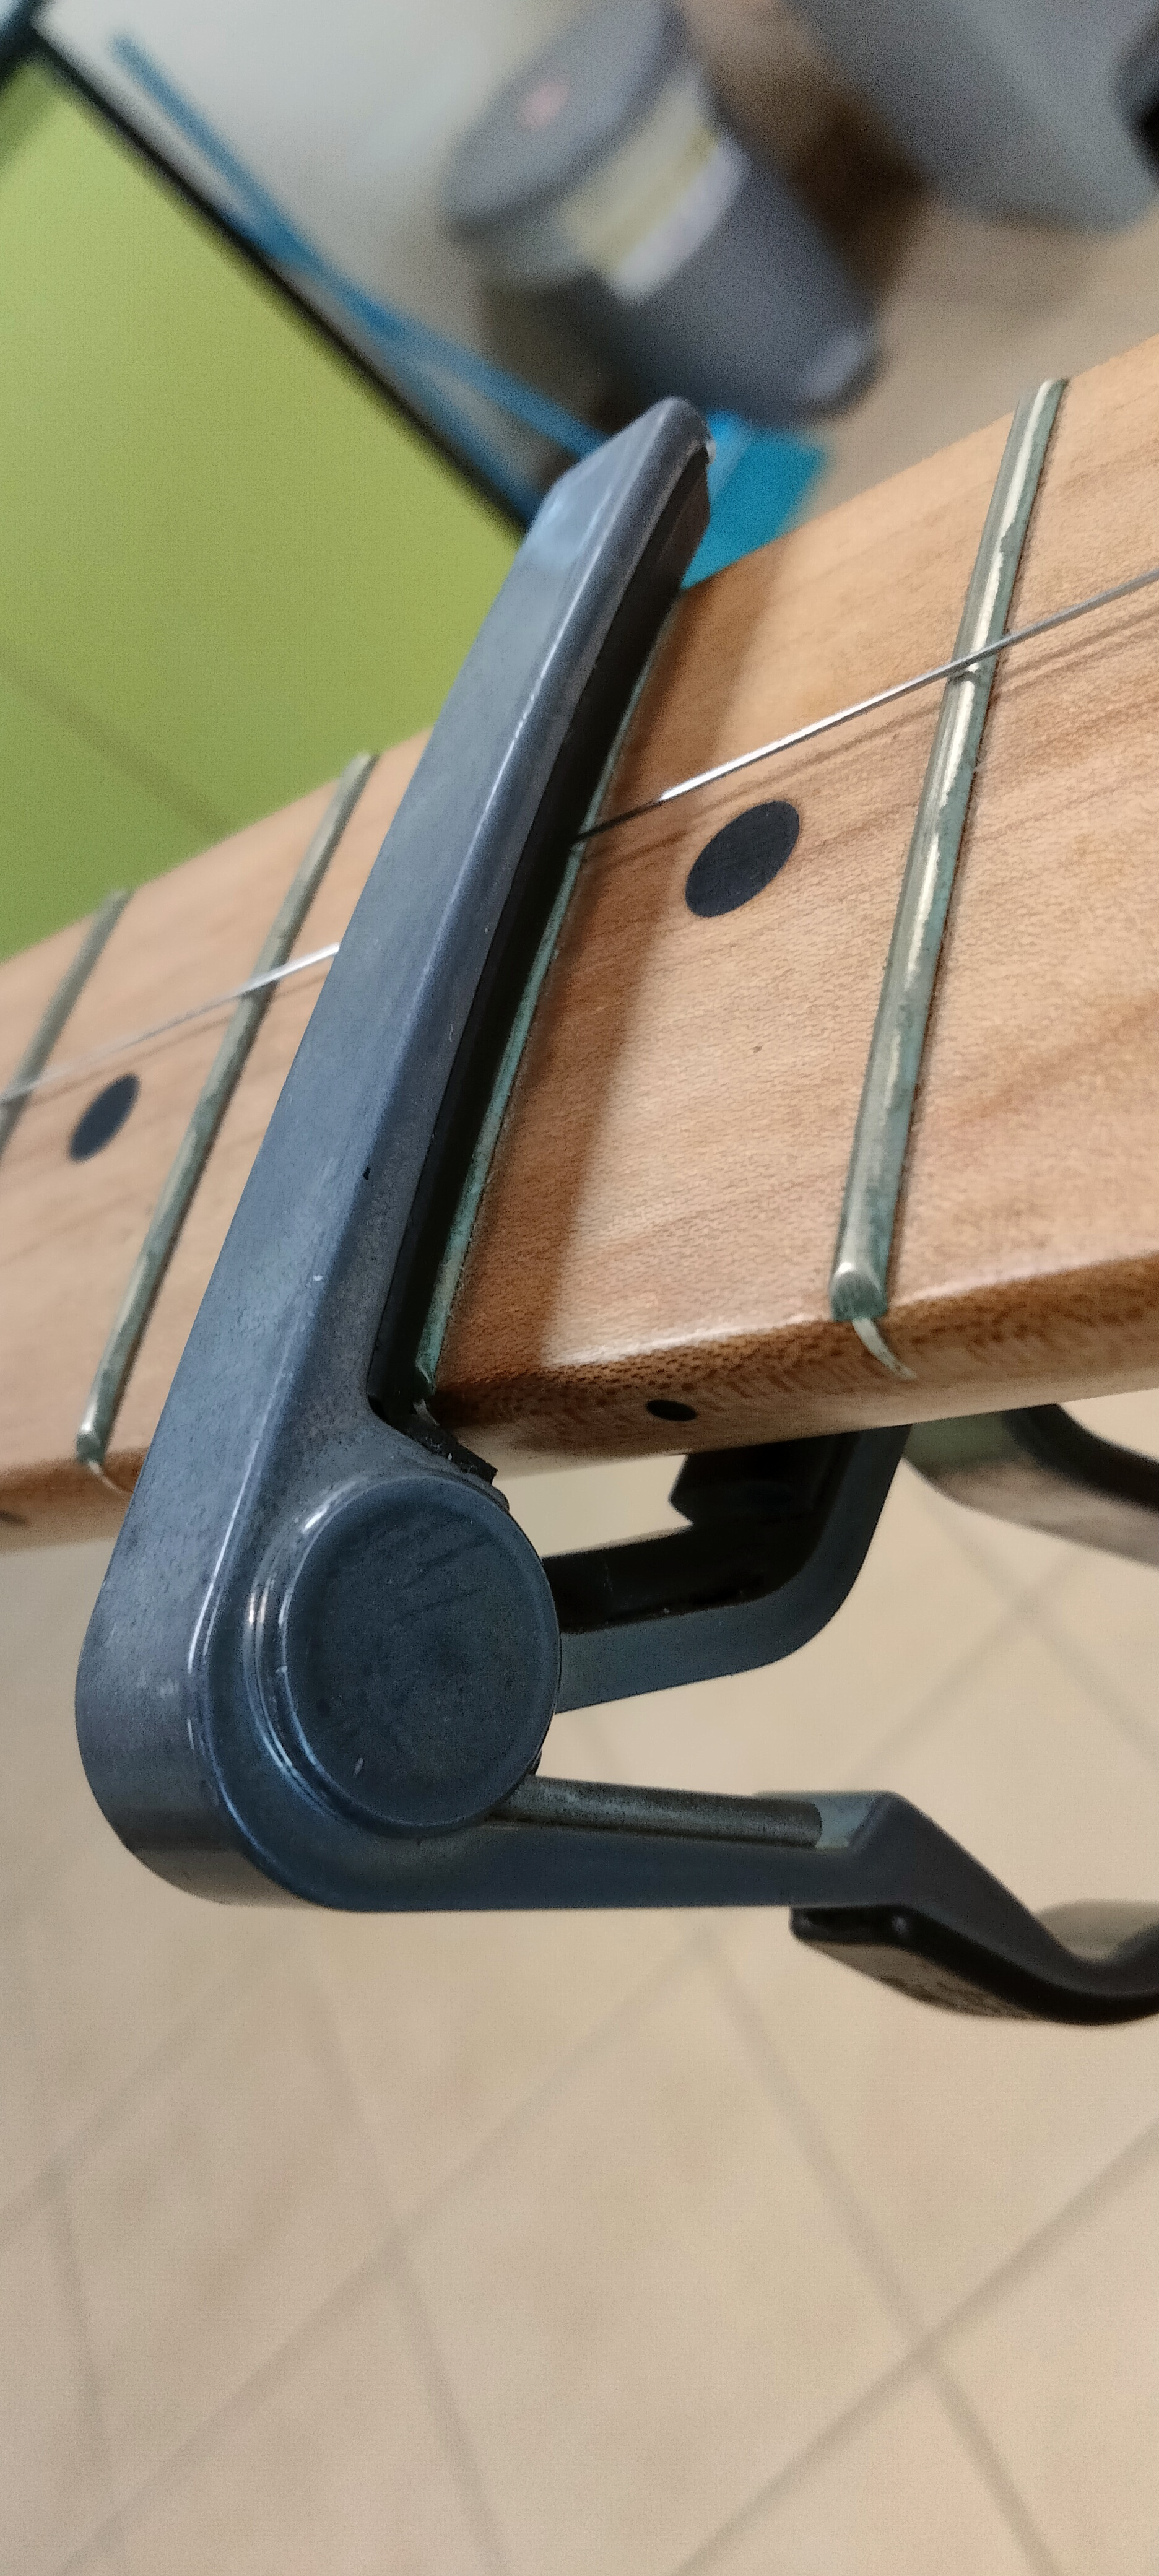
\includegraphics[angle=270, width = \textwidth]{ee/capo_on_fret.jpg}
                    \caption{Close up of capo placement. This ensures consistent pressure and contact with the string and fret} \label{fig6}
                \end{figure}
                \begin{figure}[!htb]
                    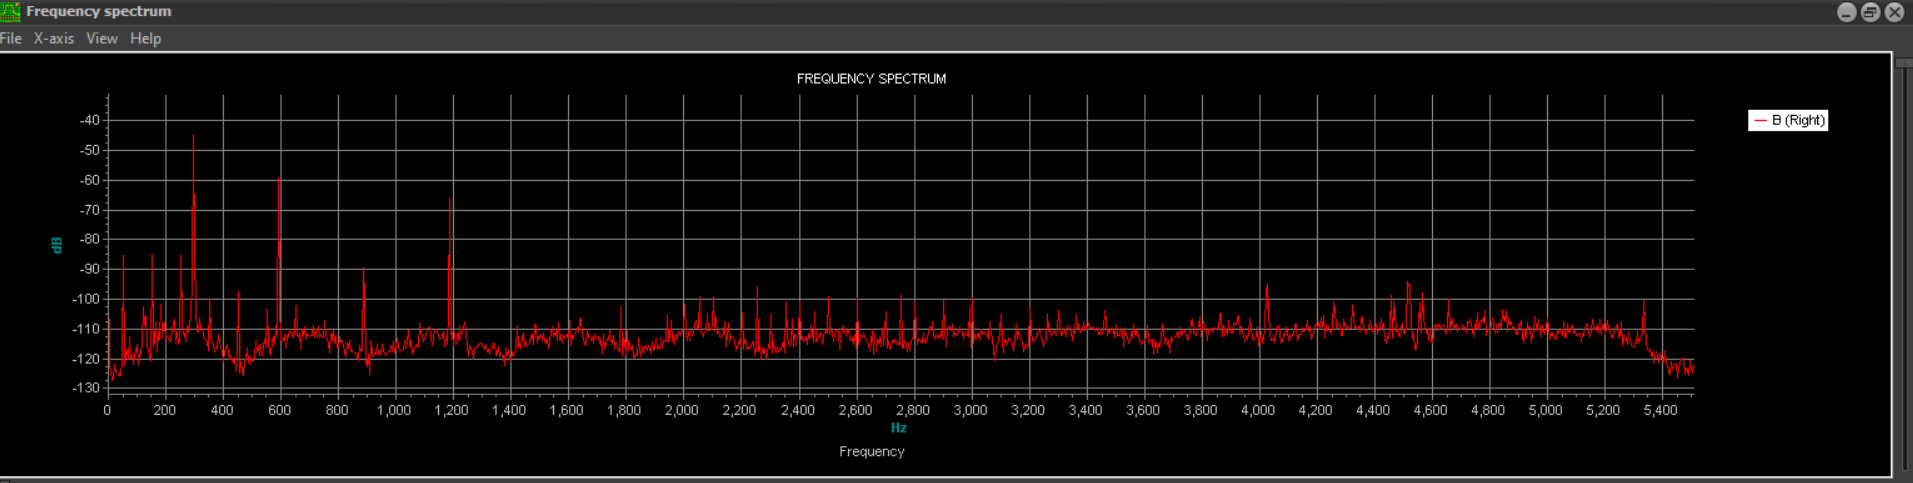
\includegraphics[width = \textwidth]{freq.png}
                    \caption{Frequency spectrum of a note in Visual Analyzer. This can be zoomed in further to accurately read peak frequency value.} \label{fig7}
                \end{figure}
        \FloatBarrier
        \subsection{Tables of results}
            \FloatBarrier  
            \subsubsection*{Table of raw data}
                \begin{figure}[!htb]
                    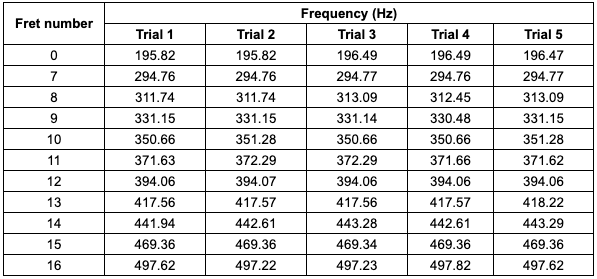
\includegraphics[width = \textwidth]{raw_table.png}
                    \captionof{table}{Raw collected data}
                \end{figure}
            \FloatBarrier
            The frequencies are taken up to 2d.p because this is the smallest the software can measure.
            \FloatBarrier
            \subsubsection*{Table of processed data}
                \begin{figure}[!htb]
                    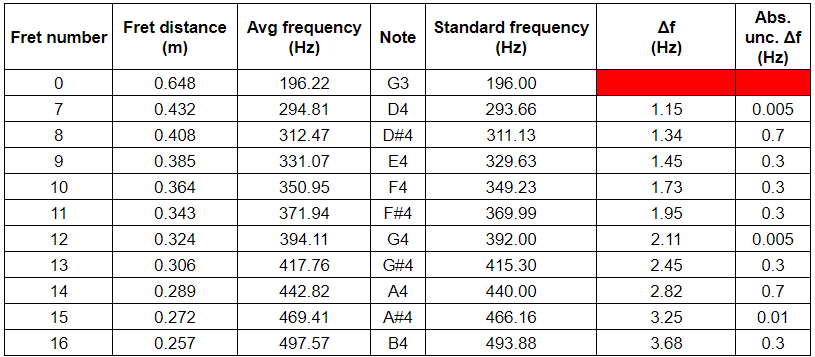
\includegraphics[width = \textwidth]{processed_table.png}
                    \captionof{table}{Table of processed data}
                \end{figure}
            \FloatBarrier
            \subsubsection*{Sample calculations}
            All example calculations are taken from values for fret 7.
            \begin{itemize}
                \item Fret distance is $l_n$, calculated from the luthier equation (\ref{eqn6})
                $$l_7 = \frac{.648}{\sqrt[12]{2^7}} = \SI{.432}{m}$$
                \item Average frequency is simply average value of the 5 trials.\\
                avg.$f = \frac{294.81 + 294.81 + 294.82 + 294.81 + 294.82 }{5} = \SI{294.81}{Hz}$
                \item Note names correspond to standard note positions on G string on a standard guitar
                \item Standard frequencies corresponding to notes. \cite{freq_chart} 
                \item $\Delta f$ is the intonation deviation at each fret, calculated as the difference between the average frequency and the standard frequency.
                $$\Delta f = 294.81 - 293.66 = \SI{1.15}{Hz}$$
                \item Absolute uncertainty of $\Delta f$ is half the range of trial values up to 1 s.f \\
                Abs. unc. of $\Delta f = (294.82-294.81)/2 = \SI{0.005}{Hz}$
            \end{itemize}
        \subsection{Analysis of results}
            \subsubsection*{Graphs}    
                After collecting the data, I can take the average value of $f_0 = \SI{196.22}{Hz}$ as the constant value of $f_0$ for Equation (\ref{eqn33}). Now I can plot the graph relating $\Delta f$ and $l_n$. The range of the graph corresponds with the distance between the nut and the highest fret of the guitar to the bridge, where the fretboard is. My guitar has 22 frets, so the position of the final fret is
                \begin{align*}
                    l_{22} = \frac{.648}{2^{\frac{22}{12}}} = \SI{0.182}{m}
                \end{align*} 
                Therefore the range I will be graphing is $\{0.182 \le l_n \le 0.648 \}$. Below is the general form of the graph.\par
                \FloatBarrier
                \begin{figure}[!ht]
                    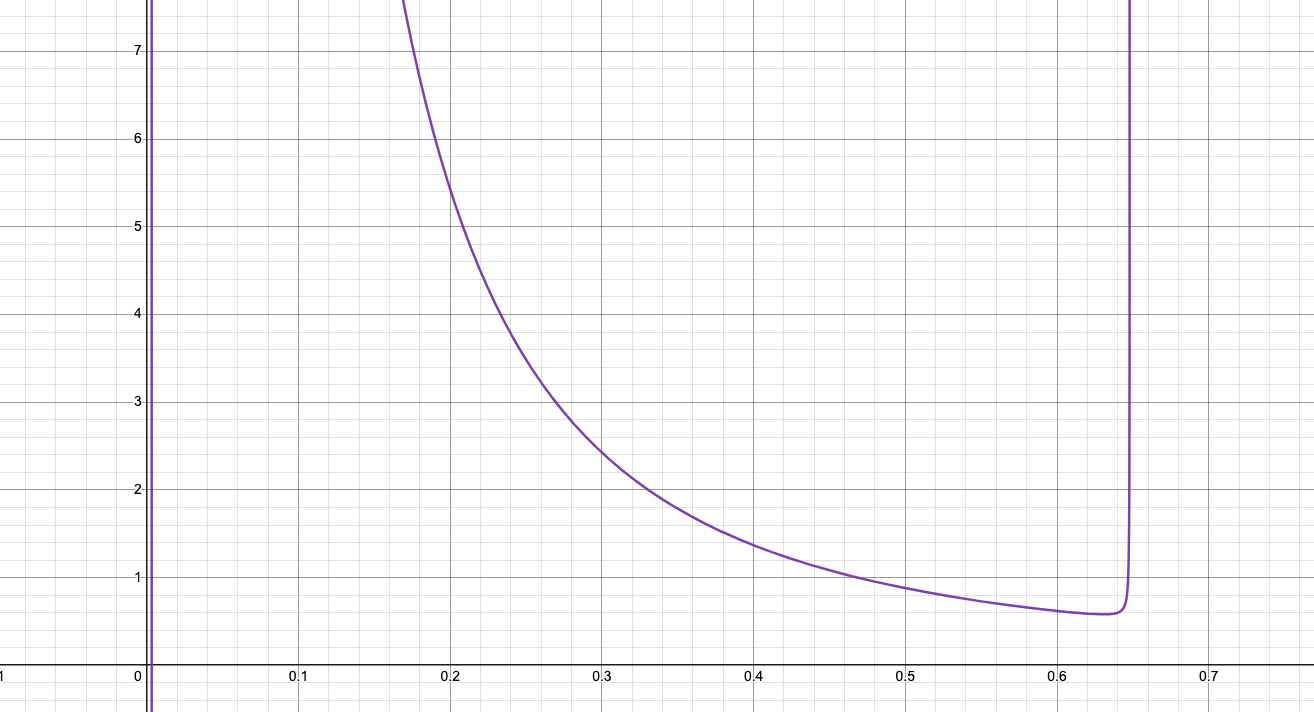
\includegraphics[width = \textwidth]{no_data_graph.png}
                    \caption{General form of the graph without data points} \label{fig8}
                \end{figure}
                \FloatBarrier
                From the graph, we can see it matches with my expectation. Overall $\Delta f$ is lower for larger $l_n$ (further from the bridge, lower frets), and increases when $l_n$ is smaller (higher frets, closer to the bridge). A noticeable thing is the function has no zero in this range, meaning everywhere you fret on the fretboard there will still be a bit of intonation error and it is impossible to achieve perfect intonation.\par
                Observing the graph, we can see there is a vertical asymptote at $l_n = l$. Mathematically this comes from equation ($\ref{eqn33}$) when the denominator of the terms inside brackets is equal to 0 ($l-l_n = 0$) (there is another asymptote at $l=0$ but this is outside of our range). At $\lim_{l_n \to l^-}$ $\Delta f$ approaches $+\infty$. This is physically impossible. My explanation of this is because of the error terms in our first order approximation. When $l \approx l_n$ (very close to the nut), $l-l_n$ is very small and on a comparable order to the nut height $b$, the approximation at (\ref{eqn26}) no longer holds because the higher order error terms will take over. This means the function will no longer accurately model the behavior of the string at that point. My physical interpretation of this phenomenon $\Delta f \to +\infty $ is because, if you try to fret very close to the nut, the "breaking angle" (angle between the fret and the string) $\theta$ of the string in Figure \ref{fig9} gets very large. Therefore the amount of force downwards needed to counteract the tension to depress the string to touch the fret is much higher, which also increases the tension of the string accordingly, which then in turn requires an even larger force to fret down, increasing the tension even more, etc. This behavior of the tension causes the frequency to rise asymptotically the closer you get to the nut. This will continue until the tension in the string is too large and the string breaks. However this doesn't happen in reality because the first fret is at $l_n = 0.612$, and you cannot fret closer to the nut than this (albeit for fretless instruments you can go as close as physically possible until the string breaks). \par
                \begin{figure}[!htb]
                    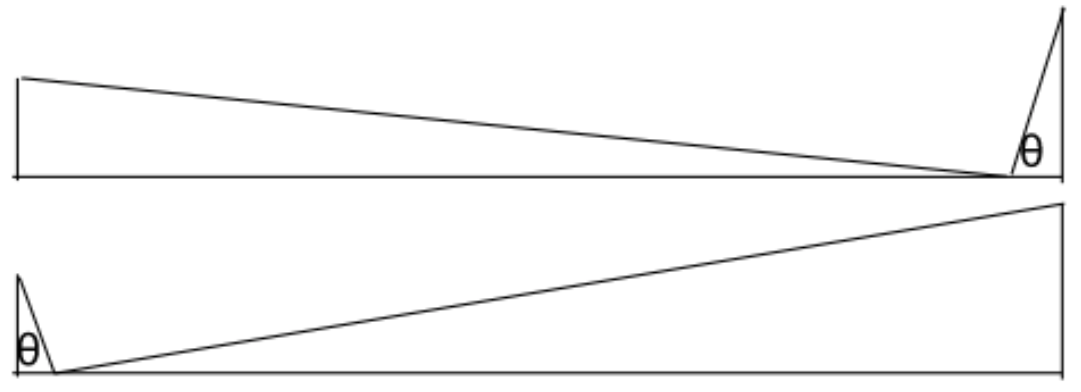
\includegraphics[width=\textwidth]{breaking_angles.png}
                    \caption{Breaking angle $\theta$ of string when fretting near the nut} \label{fig9}
                \end{figure}
                To analyze the graph further I can take the first derivative of this with respect to $l_n$. The first derivative has a zero at $l_n = 0.631$, and substituting this back into the original function we get $\Delta f = 0.598$. This is a minimum on the graph, indicating that at this point there is the least intonation error. The closest fret to this is fret 1, at $l_n = 0.612$. This shows that on the whole fretboard, the intonation error is the smallest at fret 1, and increases as you go higher up the fretboard. The local maximum is at the last fret, fret 22 at $l_n = 0.182$. Here the $\Delta f$ is 6.72 Hz, which is a relatively large intonation error. \par
                Also from the graph, the predicted $\Delta f$ at fret 7 ($l_n = 0.432$) is $\SI{1.21}{Hz}$. This deviation can be put in terms of cents, which is defined as the difference between the frequencies of two consecutive notes divided into 100 equal parts. \cite{cents} Therefore:
                \begin{align*}
                    \text{1 cent above D4} &= \frac{\text{D\#4 - D4}}{100} \\  
                    &= \frac{311.33-293.66}{100} = \SI{0.177}{Hz} 
                \end{align*}
                (Note values taken from \cite{freq_chart}) \\
                So 1.21 Hz is equivalent to $1.21/0.177 \approx 7$ cents sharp. The smallest difference in pitch human can discern is around 5-6 cents \cite{loeffler}, therefore this possibly explains why the intonation error gets noticeable from fret 7 and upwards. \par
                Now I can plot a graph with the data points and perform a regression method with a goodness-of-fit test to determine the correlation.
                \begin{figure}[!h]
                    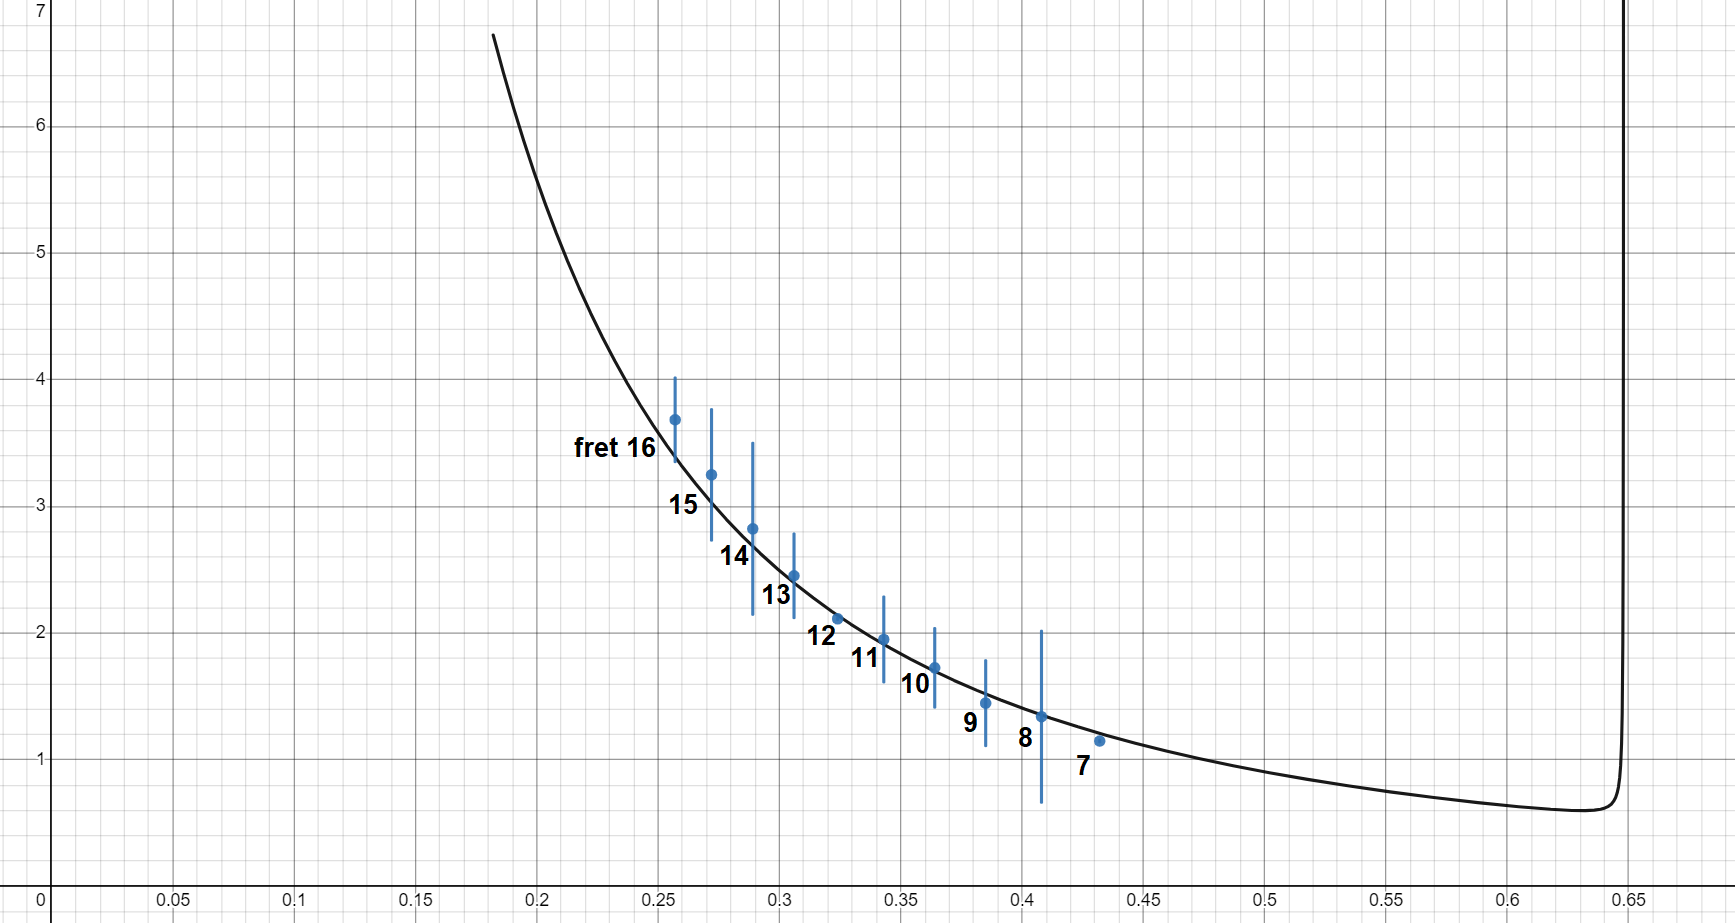
\includegraphics[width = \textwidth]{graph_with_data.png}
                    \caption{The data points with error bars} \label{fig10}
                \end{figure}
            \subsubsection*{Observation \& Analysis}
                From Figure \ref{fig10} we see the data points fit the function quite well and follow the general shape of the curve. The curve passes through all the error bars except for the data point at fret 7, which is still close to the curve but error bars are too small. A noticeable thing is that, although data points of lower frets stay pretty close to the curve, for higher frets (lower $l_n$) $\Delta f$ are quite higher than the predicted values (around frets 13-16). One possible cause of this I can think of is due to the capo placement. Because of the neck shape around this position where it connects with the body of the guitar, it is quite difficult to place the capo squarely on the fret and pressing directly down on the string. This might cause it to pull the string a bit sideway or push it down behind the fret, increasing the tension and making the frequency go up. \par
                The goodness-of-fit test I will perform on the data is the Standard Error of the Estimate (SEOE). 
                \begin{equation*}
                    \text{SEOE} = \sqrt{\frac{\sum{(Y-Y')^2}}{n}}
                \end{equation*}
                Where $Y$ is the actual value of the data, $Y'$ is the value from the function, and $n$ is the number of data points. \cite{lane} \par
                The correlation value of SEOE is essentially the standard deviation of the residual values. The closer this standard deviation is to 0, the lower the errors and the better the function fits the data (higher correlation). I choose this test because it returns a normalized result and provides a clear measure on the quality of the correlation. Performing the test on the processed data points of $\Delta f$ and $l_n$, I get a value of SEOE $= 0.130$. This is quite close to 0, indicating a low deviation of errors, so I believe the data fits the model well.
                
    \section{Conclusion \& Evaluation}
        In conclusion, the higher the fretting position, the more intonation error there is. The relationship is not a linear one but quite complicated and can be modelled with the equation (\ref{eqn33}). By plotting the collected data and performing the goodness-of-fit test, it confirms the validity of the equation. \par
        By choosing a simplified model of the guitar, it makes the calculations easier and creates a useful approximation model. However, the model doesn't take into account several factors in reality that can affect the intonation. For example, the use of a capo to simulate the fretting action of a human finger. The contact surface of a human finger on the string is very small, but that of a capo is much bigger. This can lead to more deformation of the string when using the capo and consequently an increase in tension \& frequency. Also, when fretting down on the string we don't normally press down directly on the fret like the capo, but a bit behind. This can depress the string more and lead to a higher intonation error. Another factor is the guitar neck isn't always rigid and straight like in the model but sometimes slightly bowed, either from the tension of the strings or set up by the player, which can also affect the intonation. An assumption I made in the experiment is the point of pressing down on the string would have no friction, therefore the tension increase would be distributed evenly throughout the string, but in reality the finger or the capo would have a small amount of friction that can affect the result. Another limitation of the model is it only applies to plain unwound steel strings, so it can only be used for the highest 3 strings on a guitar, but for the other 3 wound strings we would need a different model.\par

        An observation I can make from equation (\ref{eqn33}) is that it is not dependent on the gauge (thickness) of the string I use. However this conflicts with my experience, because when playing I would notice the thicker G string would exhibit more intonation shift than the thinner high E string. The explanation I have for this is due to the different $f_0$ of both strings. For E string tuned to E4, $f_0 = \SI{329.63}{Hz}$. Plotting the graph for this (Figure \ref{fig11}), we see the intonation deviation is much lower than for the G string, as expected.\par
        \FloatBarrier
        \begin{figure} [!htb]
            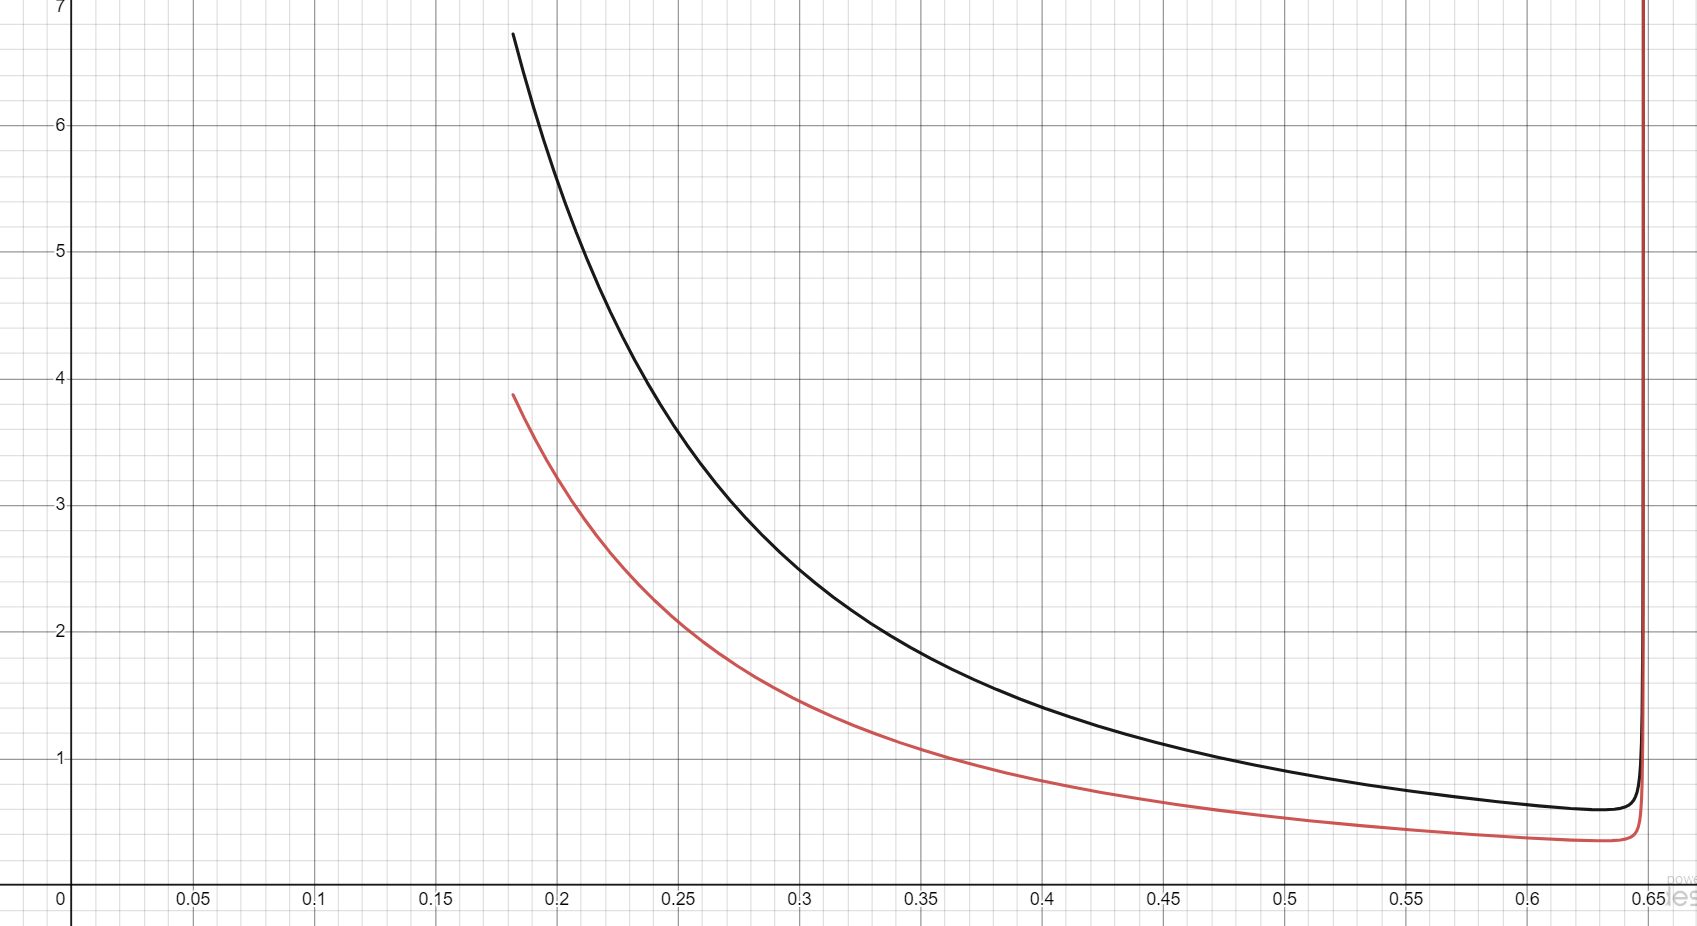
\includegraphics[width = \textwidth]{compare_graph_f.png} 
            \caption{Comparison of curve for G string (black) and high E string (red)}\label{fig11}
        \end{figure}
        Another very similar phenomenon often reported among guitar players is that, for the same string, using thicker string gauge would make the intonation a little flat overall. This means $f_0$ and every other variables are the same, but now we have negative values of $\Delta f$. This cannot be explained by the equation or shown in the graph, but I think this is caused by a different factor. For a thicker string, from equation (\ref{eqn4}), in order to tune to the same frequency $f_0$ we would need a higher tension $T$, because the linear density $\mu$ of a thicker string is larger. This higher tension would make it harder to fret down on the string (more "string resistance"), requiring more force, increasing the string tension and bending the neck slightly more. This means the string will get a little slacker and the frequency will go down. Therefore in order to minimize intonation error, it is recommended to use thinner gauge strings. However players need to take into account other factors as well when changing strings. For example it's not recommended for players with a slightly heavier playing style, because the lower resistance of thinner strings will make it more likely to be pushed sideways when fretted rather than directly down on the fret, which will also cause intonation shifts.\par
        
        From the graph of the equation relating $\Delta f$ and $l_n$ we can also evaluate the effects of changing other variables on the shape of the curve. It is impossible to have zero intonation deviation through the whole graph, but I can try ways to minimize this error. I notice the variable that has the most effect on the graph is $a$, the vertical distance between top of the bridge saddle and the frets. Simply reducing the value of $a$ by around 1 mm, bringing it from 3.3 mm down to 2 mm (\SI{2e-3}{m}) is enough to reduce the intonation shift at fret 16 down to around 1.2 Hz (Figure \ref{fig12}), which would be almost unnoticeable to the human ear. \par
        \begin{figure}[!h]
            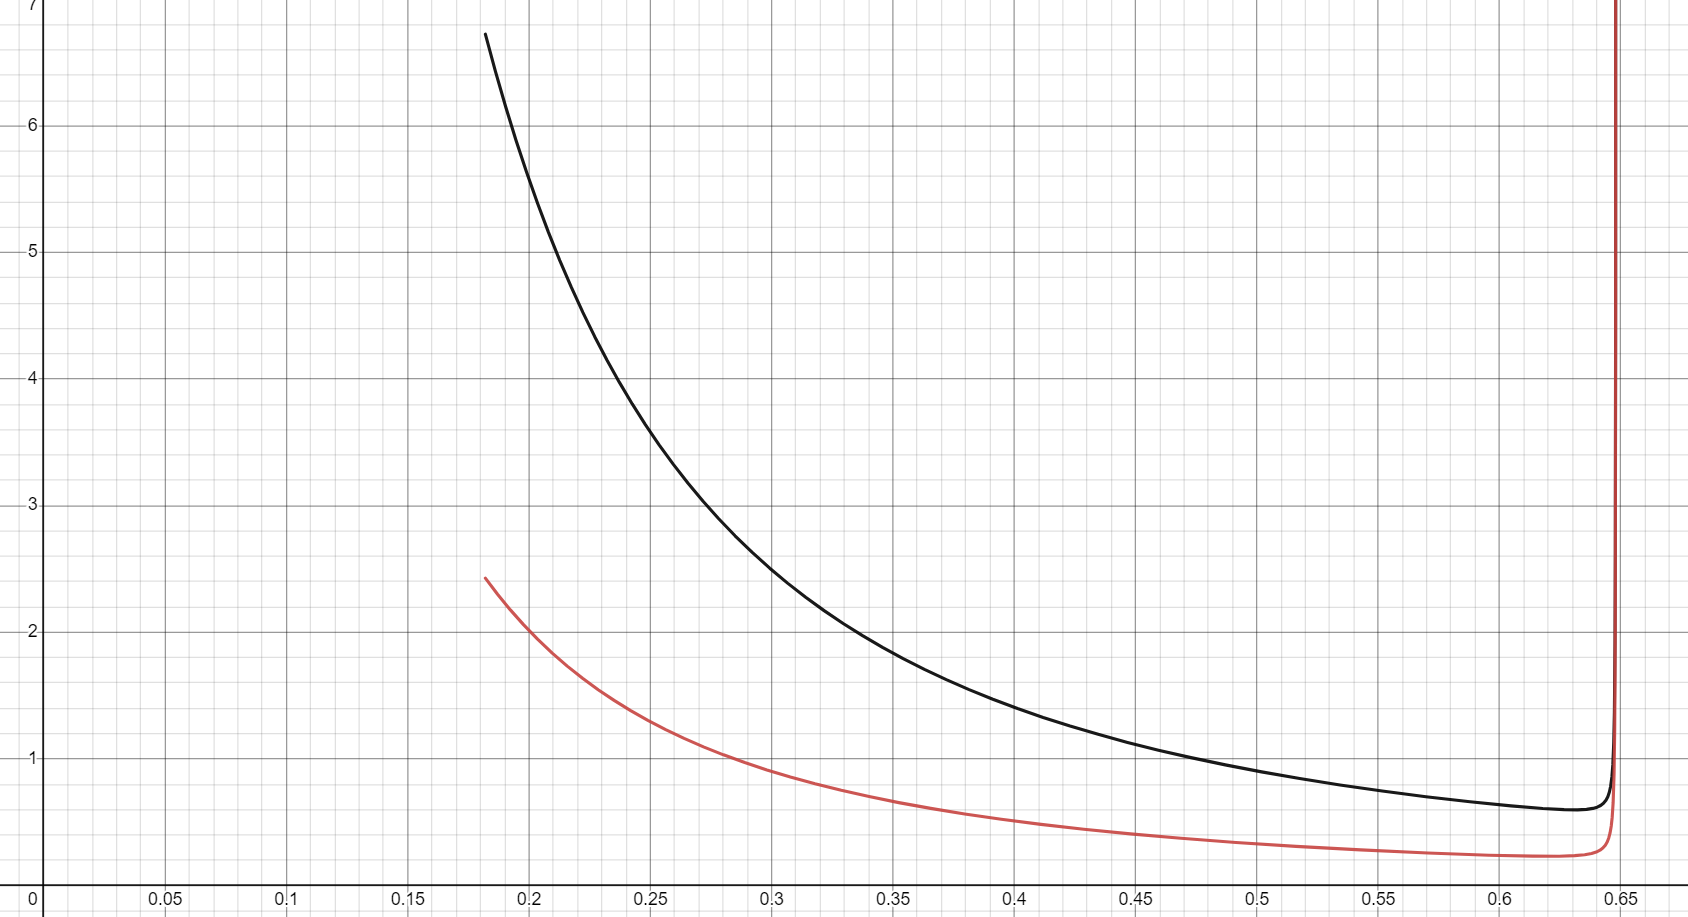
\includegraphics[width = \textwidth]{compare_graph_a.png}
            \caption{Comparison of before (black) and after changing value of $a$ (red)} \label{fig12}
        \end{figure}
        \FloatBarrier
        So a lower string action would be better for intonation. Guitar manufacturers as well as guitarists can take this into account when setting up their guitars to reduce the intonation error. However, reducing the saddle height too much will cause buzzing of the string, where the string hit against other frets when it is plucked and vibrating. This will reduce the quality of the tone and might even lead to more intonation error. Therefore a careful trial and error approach is needed when adjusting for a good intonation. \par
        
        Overall from the investigation we see that the intonation of a guitar string is a complicated variable and is affected by a lot of different factors. We cannot eliminate it completely, but there are some things we can do to control it to try and minimize the intonation shifts, such as using low gauge strings and having a low action. However I believe guitar players shouldn't worry too much about it, as I think intonation errors generally exhibit "self-correcting" behavior. This is because when a player can hear slight deviations in pitch, their fretting fingers will make micro-movements to try to compensate for this.
        \begin{thebibliography}{15}
            \scriptsize
            \bibitem[Britannica, 2023]{eqn1} Britannica, T. Editors of Encyclopaedia (2023, January 10). "wavelength. Encyclopedia Britannica". \url{https://www.britannica.com/science/wavelength}.
            
            \bibitem[OpenStax, 2016]{eqn3} OpenStax. “16.3 Wave Speed On a Stretched String.” Pressbooks, 3 Aug. 2016, \url{https://pressbooks.online.ucf.edu/osuniversityphysics/chapter/16-3-wave-speed-on-a-stretched-string}.
    
            \bibitem[Mottola]{eqn6} Mottola, R. M. “Liutaio Mottola Lutherie Information Website.” Liutaio Mottola Lutherie Information Website, \url{https://www.liutaiomottola.com/formulae/fret.htm}.
    
            \bibitem[Nemeroff, 2023]{scale} Nemeroff, Ben. "Stratocaster Buying Guide: Fender Insiders Compare 8 Electric Guitar Models." 8 Mar. 2023, \url{https://www.fender.com/articles/instruments/fender-stratocaster-buying-guide-7-strat-models-compared}.
    
            \bibitem[Suits, 1998]{freq_chart} Suits, Bryan (1998). "Frequencies of Musical Notes, A4 = 440 Hz". Physics of Music — Notes. Michigan Tech University, \url{https://pages.mtu.edu/~suits/notefreqs}.
            
            \bibitem[Polak et al., 2018]{polak} Polak, Robert D., et al. “Determining Young’s Modulus by Measuring Guitar String Frequency.” The Physics Teacher, American Association of Physics Teachers, Jan. 2018, \url{https://doi.org/10.1119/1.5021447}.
    
            \bibitem[ASTM A228 Steel (UNS K08500)]{astm} ASTM A228 Steel (UNS K08500), \url{https://www.matweb.com/search/datasheet_print.aspx?matguid=4bcaab41d4eb43b3824d9de31c2c6849}.
    
            \bibitem[StewMac.com]{stewmac} StewMac, “String Action Gauge Instructions.” \url{https://www.stewmac.com/video-and-ideas/online-resources/neck-building-and-repair-and-setup/string-action-gauge-instructions}.
    
            \bibitem[VA2020 Website]{va20} \url{https://www.sillanumsoft.org/}.
    
            \bibitem[Suits, 1998]{cents} Suits, Bryan (1998). "Making Sense of Cents". Physics of Music — Notes. Michigan Tech University, \url{https://pages.mtu.edu/~suits/cents}.
    
            \bibitem[Loeffler, 2006]{loeffler} Loeffler, D.B. (April 2006). Instrument Timbres and Pitch Estimation in Polyphonic Music (Master's). Department of Electrical and Computer Engineering, Georgia Tech. \url{https://web.archive.org/web/20071218232401/http://etd.gatech.edu/theses/available/etd-04102006-142310/}
    
            \bibitem[Lane]{lane} Lane, David M. "Standard Error of the Estimate.", Online Stat Book, \url{https://www.onlinestatbook.com/2/regression/accuracy.html.}
    
        \end{thebibliography}

    \end{flushleft}

\end{document}